\documentclass{standalone}
\usepackage{pgfplots, amssymb}
\pgfplotsset{
  compat=1.18, 
  trig format=rad, 
  ticklabel style = {font=\footnotesize},
  axis equal image,
}

\begin{document}
  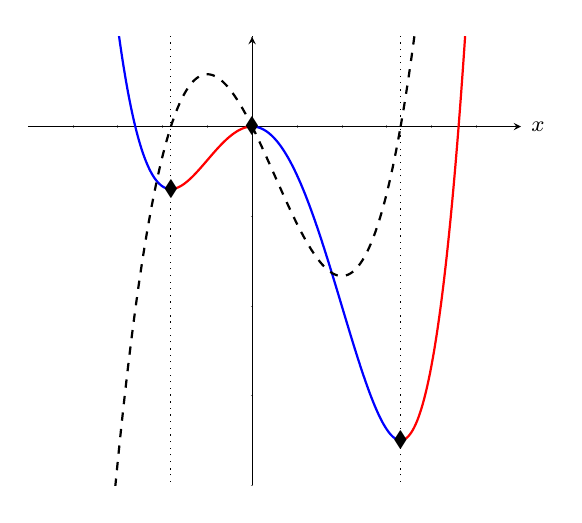
\begin{tikzpicture}
    \begin{axis}[
      axis lines=middle,
      % width=5in, height=5in,
      ymin=-8, ymax=2,
      xmin=-5, xmax=6,
      % ymin=-4, ymax=4,
      xlabel={\footnotesize \(x\)},
      xlabel style={at={(ticklabel* cs:1)}, anchor=west},
      % ylabel={\footnotesize \(y\)},
      % ylabel style={at={(ticklabel* cs:1)}, anchor=south},
      axis line style = {very thin},
      % xticklabels={,,},
      yticklabels={,,},
      xtick={-4,-3,-2,-1,0,1,2,3,4,5},
      xticklabels={,,,\phantom{-1},,,\phantom{2},},  % use phantom to force the plot to have the same dimension as the concavity plot.
      samples=500,
      % grid=both,
      % grid style={line width=.2pt, draw=gray!20},
      % minor tick num=1, 
      smooth,
      thick,
      no markers,
      tickwidth={1pt},
      ]
      % sage: f(x) = ((x+1)*(x-2)).integrate(x).integrate(x)
      \addplot[no markers, smooth, domain=-4:-1.81174, blue] {1/12*x^4 - 1/6*x^3 - x^2};
      \addplot[no markers, smooth, domain=-1.81174:0, red] {1/12*x^4 - 1/6*x^3 - x^2};
      \addplot[no markers, smooth, domain=0:3.31174, blue] {1/12*x^4 - 1/6*x^3 - x^2};
      \addplot[no markers, smooth, domain=3.31174:6, red] {1/12*x^4 - 1/6*x^3 - x^2};
      \node at (-1.81174,-1.39341) {\footnotesize \(\blacklozenge\)};
      % \node[below right] at (-1.81174,-1.39341) {\footnotesize \(A\)};
      \node at (0.00000,0.00000) {\footnotesize \(\blacklozenge\)};
      % \node[above right] at (0.00000,0.00000) {\footnotesize \(B\)};
      \node at (3.31174,-6.99721) {\footnotesize \(\blacklozenge\)};
      % \node[below right] at (3.31174,-6.99721) {\footnotesize \(C\)};

      \addplot[dashed, no markers, smooth, domain=-4:-1.81174] {1/3*x^3 - 1/2*x^2 - 2*x};
      \addplot[dashed, no markers, smooth, domain=-1.81174:0] {1/3*x^3 - 1/2*x^2 - 2*x};
      \addplot[dashed, no markers, smooth, domain=0:3.31174] {1/3*x^3 - 1/2*x^2 - 2*x};
      \addplot[dashed, no markers, smooth, domain=3.31174:6] {1/3*x^3 - 1/2*x^2 - 2*x};

      \addplot[dotted, thin] coordinates { (-1.81174, -10) (-1.81174, 10) };
      \addplot[dotted, thin] coordinates { (0, -10) (0, 10) };
      \addplot[dotted, thin] coordinates { (3.31174, -10) (3.31174, 10) };
    \end{axis}
  \end{tikzpicture}
\end{document}
